\subsection{Gestion des données}
\label{Donnees}

\subsubsection{Des données à analyser}

\paragraph{}Dans la tâche d'expérimentation réalisée par les chercheurs, certaines données sont recueillies pour être analysées. Ces données regroupent :
\begin{description}
\item[Les hits :] à chaque fois qu'une cible est trouvée. Cette donnée est enregistrée sous la forme d'un pourcentage de hits réussi sur toutes les cibles apparues.
\item[Les FA :] lorsque le sujet pense avoir vu une cible alors qu'il n'y en a pas. Cette donnée est enregistrée sous la forme d'un pourcentage de FA sur tous les distracteurs apparus.
\item[Les miss :] lorsque le sujet rate une cible. Cette donnée est l'inverse des hits.
\item[Le dprime :] la sensibilité du sujet pour identifier la cible des distracteurs. Voici le calcul de la valeur du dprime : \[NormeInverse(PourcentageHits) - NormeInverse(PourcentageFA)\]
\end{description}

\newpage
\paragraph{}Ces données sont propres à chaque sujet et sont analysées par session. On peut ainsi voir l'impact de l'entrainement sur le sujet et comparer son évolution par rapport
aux autres sujets. J'ai pu participer à la tâche d'entrainement en tant que sujet afin de bien comprendre son fonctionnement. \`{A} chaque session, mes performances se
sont améliorées. Voici mes résultats sur 5 sessions :

\begin{figure}[H]
    \begin{center}
    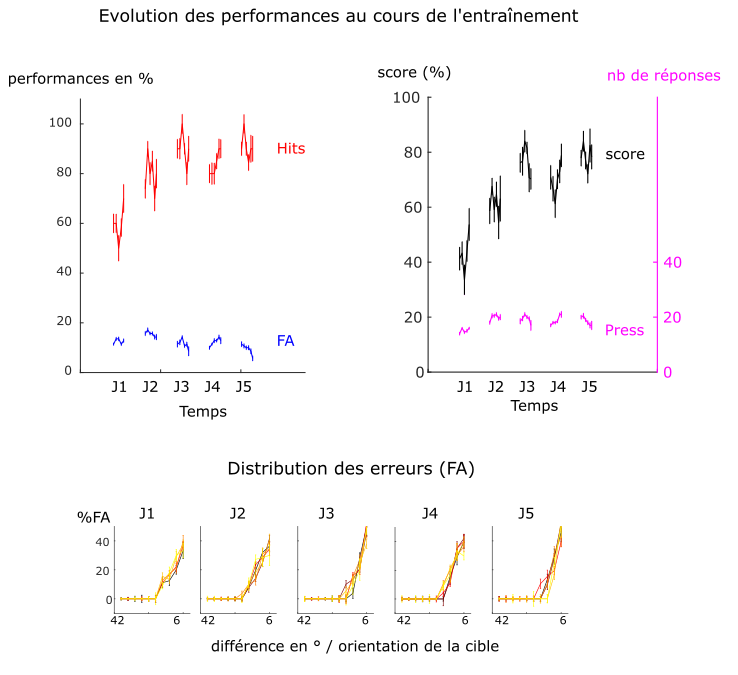
\includegraphics[width=11cm]{cptPerformance.png}
    \end{center}
    \caption{L'évolution de mes performances sur la tâche de CPT sur 5 sessions}
\label{CptPerformance}
\end{figure}

\paragraph{}Un des objectifs du jeu est d'obtenir ces données à partir des performances des joueurs. De cette façon, les chercheurs auront accès à un nombre assez conséquent de
données à analyser. Le premier problème qui s'est posé est celui de la conservation de données personnelles. En effet, conserver ce type de données nécessite de monter un dossier
auprès de la \gls{CNIL}, ce qui implique une procédure assez longue (plusieurs mois, voire plus d'un an). C'est pourquoi nous avons fait le choix d'anonymiser les données recueillies.
Parmi les données à recueillir, les informations de connexion étaient les seules permettant d'identifier formellement un joueur. Nous avons donc choisi de créer un hash à partir du
login et du mot de passe et nous l'utilisons afin de différencier les joueurs.

\paragraph{}Un autre problème s'est posé dans la gestion de la progression des joueurs. Pour des raisons de sécurité informatique, \emph{Sylvain Maurin} préférait éviter d'envoyer des
données autres que le jeu en lui-même aux joueurs. Il était donc nécessaire de trouver des solutions pour que la connexion du joueur et la sauvegarde de sa progression soient présent
sans lui renvoyer d'informations.

Concernant la connexion, nous sommes partis du principe que le joueur devait bien retenir ses identifiants. Si son identification est connue, nous ajoutons ses données à son profil,
sinon, nous créons un nouveau profil de joueur.

\begin{figure}[H]
    \begin{center}
    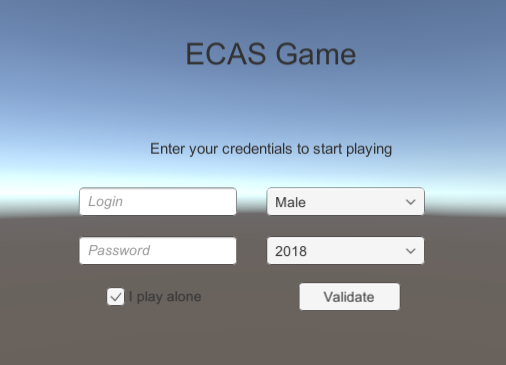
\includegraphics[width=10cm]{login-screen.png}
    \end{center}
    \caption{Ecran de connexion du joueur}
\label{LoginScreen}
\end{figure}

\paragraph{}Pour la sauvegarde de la progression du joueur, nous pensons extraire du jeu un fichier texte qui permet de savoir où le joueur en est dans le jeu. Lorsque celui-ci crée une
nouvelle session de jeu (à sa connexion), il pourra importer ce fichier texte, et le jeu chargera sa progression.

\subsubsection{Méthode d'envoi des données}

\paragraph{}Pour envoyer les données, nous avons choisi d'envoyer des logs à un serveur web Apache. Ces logs sont enregistrées dans un fichier texte sur le serveur. Les données sont
envoyées à différents moments lorsqu'un joueur joue :
\begin{description}
\item[Lors de la connexion :] Un nouveau profil de joueur est créé s'il n'existe pas encore. Une nouvelle session de jeu est créée pour connaitre la date et si le joueur joue seul.
\item[Lors de la création d'un partie :] Une nouvelle partie est créée avec la date et le jeu choisi.
\item[Lors d'évènements dans le jeu :] On doit envoyer chaque hit, miss, distracteur apparu, FA et la valeur du dprime régulièrement avec le timestamp pour chacun afin de connaitre la
chronologie des évènements dans le jeu pour une meilleure analyse
\end{description}

\paragraph{}Les données sont envoyées sous une forme semblable à une url : c'est une chaine de caractère contenant des données séparées par des "/". Voila la forme de ces url pour
envoi de données :
\begin{description}
    \item[Création d'un joueur :] ecas / RegisterUser / \textit{hashPlayer} / \textit{yearBirth} / \textit{sexe}
    \item[Création d'une session :] ecas / CreateSession / \textit{hashPlayer} / \textit{hashSession} / \textit{timestamp} / \textit{isAlone}
    \item[Fermeture d'une session :] ecas / CloseSession / \textit{hashSession} / \textit{timestamp}
    \item[Création d'une partie :] ecas / CreateParty / \textit{hashSession} / \textit{hashParty} / \textit{timestamp} / \textit{game}
    \item[Fermeture d'une partie :] ecas / CloseParty / \textit{hashParty} / \textit{timestamp}
    \item[Enregistrement d'un hit :] ecas / RegisterHit / \textit{hashParty} / \textit{timestamp} / \textit{reactionTime} / \textit{tube}
    \item[Enregistrement d'un miss :] ecas / RegisterMiss / \textit{hashParty} / \textit{timestamp} / \textit{tube}
    \item[Enregistrement d'un distracteur :] ecas / RegisterDistractor / \textit{hashParty} / \textit{timestamp} / \textit{tube}
    \item[Enregistrement d'une FA :] ecas / RegisterFA / \textit{hashParty} / \textit{timestamp} / \textit{tube}
    \item[Enregistrement du dprime :] ecas / RegisterDPrime / \textit{hashParty} / \textit{timestamp} / \textit{value}
\end{description}

\paragraph{}Ces url sont envoyée au serveur web. Il suffit ensuite de les récupérer, puis de les analyser pour extraire les données voulues. La figure \ref{DataSending} montre l'envoi
des données depuis le jeu jusqu'à leur extraction.

\begin{figure}[H]
    \begin{center}
    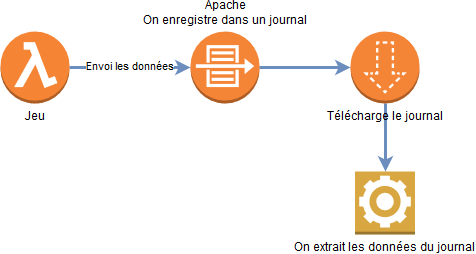
\includegraphics[width=10cm]{diagram_data_sending.png}
    \end{center}
    \caption{Diagramme d'envoi des données}
\label{DataSending}
\end{figure}


\subsubsection{Récupération et traitement des données}

\paragraph{}Nous avons décidé pour traiter les données de créer un parseur en \emph{Rust}\footnote{\url{https://www.rust-lang.org/fr-FR/}}. Cela m'a permis d'apprendre un peu ce
langage que je ne connaissais pas. Nous avons l'avons utilisé pour plusieurs raisons:
\begin{itemize}
    \item C'est un langage qui interdit au travers de son compilateur beaucoup d'erreur. Cette particularité nous permet d'assurer que les chercheurs ou futurs 
    développeur travaillant sur ce projet ne pourrons pas écrire un code incorrect facilement. En contrepartie, l'évolution de cet extracteur sera plus longue.
    \item C'est un langage naturellement multiplateforme.
    \item C'est un langage compilé qui fournit un exécutable après construction. Il n'y a donc nul besoin d'une "machine virtuelle" tel que la \emph{JVM} pour 
    Java ou l'\emph{interpréteur de Python} pour Python.
\end{itemize}


\paragraph{}Ce parseur récupère les logs du serveur Apache et permet de créer un fichier JSON utilisable par les chercheurs. Un énumérateur permet de déterminer le comportement du
parseur selon le type de donnée reçu. Il analyse le "verbe" contenu dans l'url (le 2\up{ème} élément), puis traite les données afin d'en faire une structure de données qui contient
les utilisateurs, leurs sessions, leurs parties et leurs données.

\begin{figure}[H]
    \begin{center}
    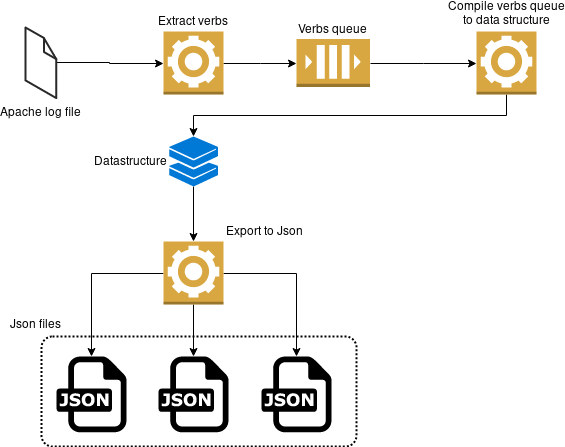
\includegraphics[width=10cm]{parser_internal.png}
    \end{center}
    \caption{Fonctionnement du parseur de données}
\label{DataParser}
\end{figure}

\paragraph{}Pour créer le fichier JSON, nous avons utilisé la bibliothèque \emph{Serde}\cite{JSONRUST} disponible sur Github. Grâce à cette bibliothèque, le parseur crée plusieurs
fichiers. Un premier fichier répertorie tous les joueurs de notre jeu avec leur année de naissance et leur sexe. Ensuite, un fichier est créé pour chaque joueur et contient toutes
les données envoyées lors de ses temps de jeu, à savoir les sessions, les parties, les données de chaque partie comme le dprime ...